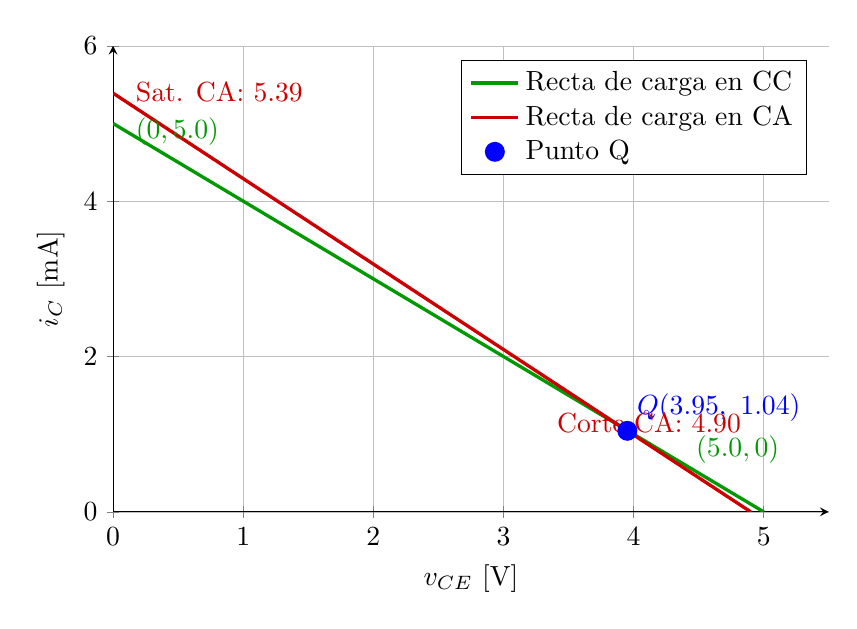
\begin{tikzpicture}
  \begin{axis}[
    width=0.88\textwidth,
    height=7.5cm,
    xlabel={$v_{CE}\ [\mathrm{V}]$},
    ylabel={$i_C\ [\mathrm{mA}]$},
    xmin=0, xmax=5.5,
    ymin=0, ymax=6.0,
    grid=both,
    grid style={line width=.1pt, draw=gray!30},
    major grid style={line width=.2pt,draw=gray!50},
    axis lines=left,
    legend pos=north east,
    legend cell align={left},
    every axis plot/.append style={very thick}
  ]
    % Recta de carga estatica (CC)
    \addplot[domain=0:5.0, color=green!60!black, samples=2] {5.0 - x};
    \addlegendentry{Recta de carga en CC }

    % Recta de carga dinamica (CA)
    \addplot[domain=0:4.90, color=red!80!black, samples=2] {1.043 + (3.952 - x)/0.90909};
    \addlegendentry{Recta de carga en CA }

    % Punto Q de reposo
    \addplot[only marks, mark=*, mark size=3pt, color=blue] coordinates {(3.952, 1.043)};
    \addlegendentry{Punto Q}

    % Anotaciones
    \node[above right, text=blue] at (axis cs:3.952, 1.043) {$Q(3.95\V,\ 1.04\mA)$};
    \node[above, text=green!60!black] at (axis cs:4.8, 0.5) {$(5.0\V, 0\mA)$};
    \node[right, text=green!60!black] at (axis cs:0.1, 4.9) {$(0\V, 5.0\mA)$};
    \node[above left, text=red!80!black] at (axis cs:4.9, 0.9) {Corte CA: $4.90\V$};
    \node[right, text=red!80!black] at (axis cs:0.1, 5.4) {Sat. CA: $5.39\mA$};
  \end{axis}
\end{tikzpicture}
